\documentclass[11pt]{article}
\usepackage{amsmath, amssymb, geometry, hyperref, graphicx}
\geometry{a4paper, margin=1in}

\title{Work Stream 6: Measure Theory, Genericity, and the Codimension of the Blow-up}
\author{MechanicaFluidorum Program \& Community Contributors}
\date{September 2026}

\begin{document}
\maketitle

\section{Introduction}
A profound discussion between mathematicians in the community (\texttt{u/Spidero0w0o}, \texttt{u/cowgod42}, \texttt{u/ComprehensiveWash958}) centered on how to rigorously describe the ``unlikeliness'' of the singularity using measure theory on infinite-dimensional Hilbert spaces ($H^s(\mathbb{R}^3)$).

\section{Shyness and Prevalence}
Because Lebesgue measure does not exist in infinite dimensions, we apply the Hunt--Sauer--Yorke definition of \emph{shyness}. We hypothesize that the set of initial conditions (or forces) leading to the OpenAI blowup is a shy set.

An earlier draft supported this by the conditioning of the $5 \times 5$ linear system that matches the five radial moments of the inner and outer profiles (Proposition~B.8 and Eqs.~(5.10)--(5.11) of the OpenAI Navier--Stokes paper). The raw, dimensional matrix $A$ has a condition number growing as $\kappa(A) \sim X_R^{7.75}$, reaching $\sim 10^{28}$ at $X_R = 1000$. This is a non-dimensionalization artifact: $A$ mixes entries spanning $X_R^0$ to $X_R^8$, and after diagonal scaling $A = DBD$ the dimensionless system has $\kappa(B) \approx 4.11 \times 10^5$, independent of $X_R$ and numerically benign (see \texttt{OpenAI\_NSE\_Verification.tex}, \S3). The condition number of a linear system used to \emph{choose parameters in a proof} is in any case not a dynamical instability of the flow, and it says nothing about shyness. The measure-theoretic hypothesis therefore stands on its own and needs a different tool.

\begin{figure}[ht]
    \centering
    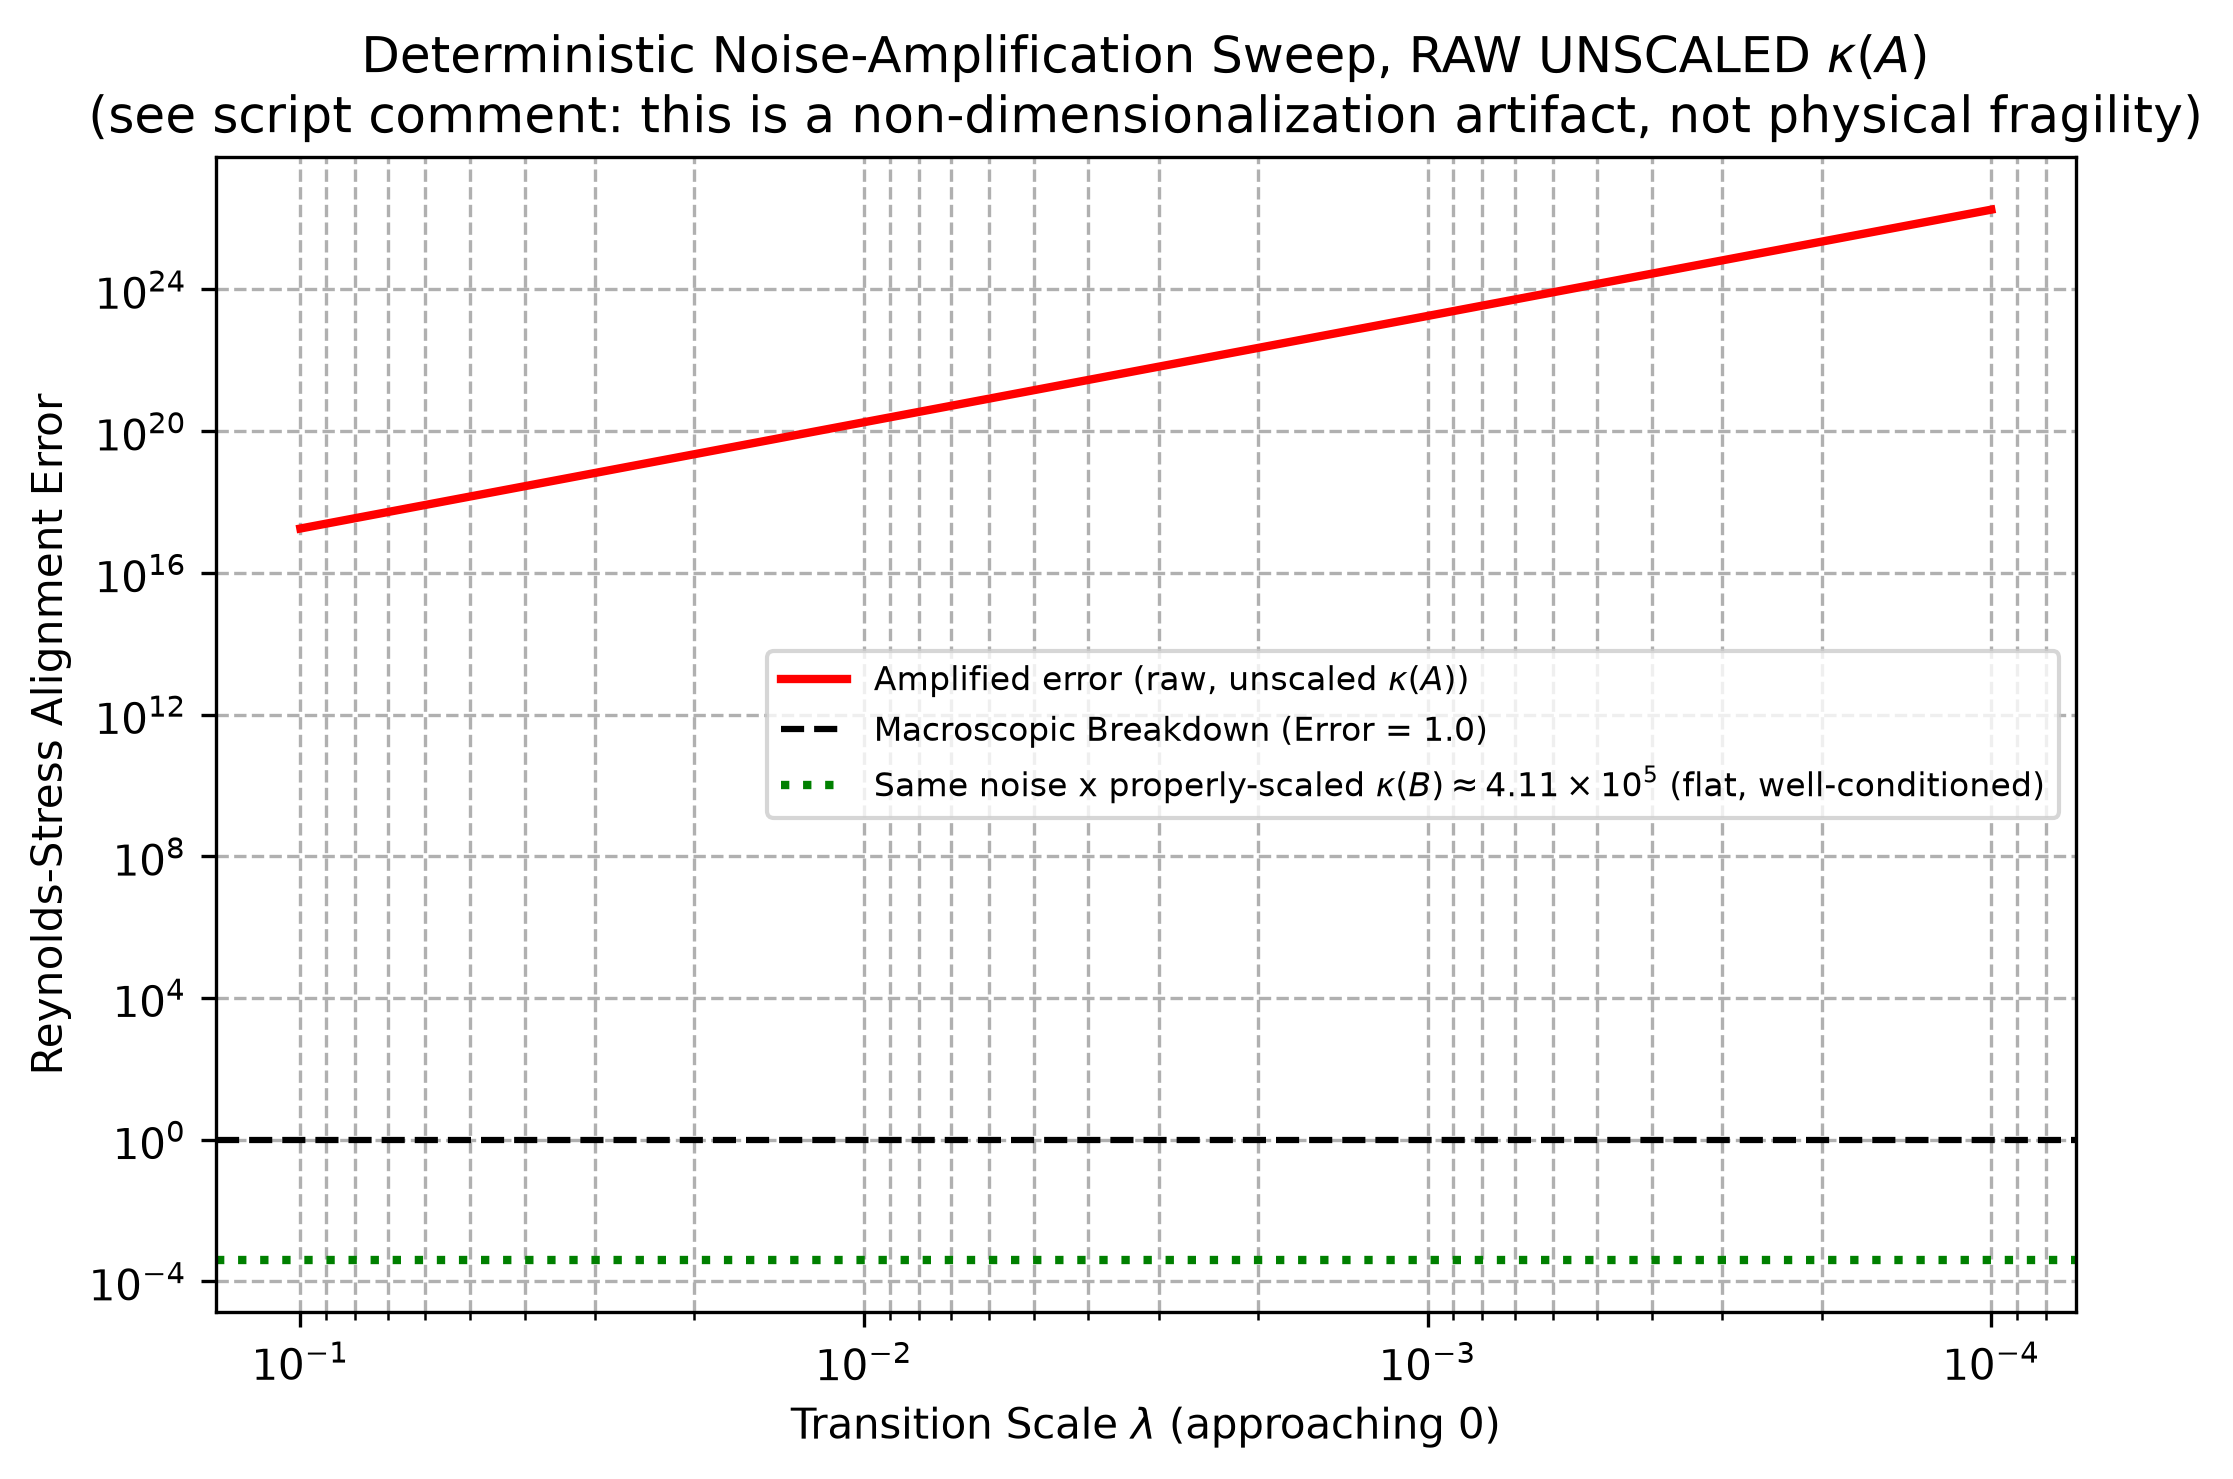
\includegraphics[width=0.8\textwidth]{jacobian_monte_carlo.png}
    \caption{Deterministic noise-amplification sweep of the raw, unscaled moment-matching matrix $A$ as a function of the transition scale $\lambda$. The apparent amplification of a $10^{-9}$\,m/s perturbation to order one is a property of the unscaled coordinates; the properly non-dimensionalized system (green line, $\kappa(B) \approx 4.11 \times 10^5$) shows none of it. The figure is retained only to document why the earlier ``$10^{28}$ fine-tuning'' reading was withdrawn.}
    \label{fig:jacobian}
\end{figure}

\section{The Rigorous Version: Codimension}
The precise meaning of ``non-generic'' for a self-similar blow-up is its \emph{codimension}: linearize the leading-order self-similar profile in similarity variables and count the unstable eigenmodes beyond those generated by the symmetries of the equation (space and time translations, scaling). A profile with $m$ genuinely unstable directions is reached from a codimension-$m$ set of nearby data and forces; $m = 0$ is a stable, hence generic, blow-up. This is exactly the question that computer-assisted and neural-network methods have answered for Boussinesq and Euler profiles: Chen and Hou established a stable nearly self-similar blow-up with smooth data~\cite{ChenHou2022}, and Wang et al. discovered families of \emph{unstable} self-similar singularities with a definite number of unstable modes~\cite{Wang2025}. A finite, nonzero $m$ for the OpenAI core would give ``shy'' a concrete meaning; it would \emph{not} make the blow-up irrelevant, since unstable self-similar solutions still organize transient dynamics. Computing $m$ for the linearized OpenAI profile is the open problem this work stream now proposes in place of the condition-number argument.

\begin{thebibliography}{9}
\bibitem{ChenHou2022} J. Chen, T.~Y. Hou, ``Stable nearly self-similar blowup of the 2D Boussinesq and 3D Euler equations with smooth data,'' arXiv:2210.07191, 2022.
\bibitem{Wang2025} Y. Wang et al., ``Discovery of unstable singularities,'' arXiv:2509.14185, 2025.
\end{thebibliography}

\section*{Acknowledgments}
We thank the rigorous mathematical community on \texttt{r/math} and \texttt{r/FluidMechanics} for highlighting the need for infinite-dimensional measure theory.

\end{document}
